%!TEX root = ../report.tex

\section{Technik}

Generell geht es darum Bewegungsabläufe in Bezug auf Geschwindigkeit und/oder Genauigkeit zu optimieren. Dadurch lassen sich Konditionelle Fähigkeiten optimal ausnutzen, Belastungen reduzieren und das Verletzungsrisiko senken.

\subsection{Begriffe \& Systematik}

Technik ist eine Sammelbezeichnung für eine Reihe technischer Fertigkeiten eines Sportlers/einer Sportart. Eine technische Fertigkeit ist eine erprobte, zweckmäßige und effektive Bewegungsfolge zur Lösung einer definierten Aufgabe in Sportsituationen. Beispiel: Pritschen ist erprobte Bewegungsabfolge der Aufgabe ``Zuspielen'' und teil der technischen Fertigkeiten eines Volleyballers.

Eigenschaften der Technik:
\begin{itemize}
    \item Individualitätseigenschaft: Eindeutige Identifizierung von Weltklasseathleten auf Basis ihrer individuellen Technik
    \item Stabilitätseigenschaft: Technische Fertigkeiten sind hochgeübte Bewegungsfolgen die erst nach Jahren beherrscht werden
    \item Variabilitätseigenschaft: Biomechanische Messungen zeigen immer Variabilitäten, Keine Bewegung entspricht exakt einer anderen und Fähigkeit zur Anpassung der Bewegung während der Ausführung wichtig
\end{itemize}

Es gibt verschiedene Möglichkeiten die Technik zu unterteilen.
Beispiele:
\begin{itemize}
    \item Elementare Fähigkeiten vs. komplexe Sportspezifische Fertigkeiten
    \item Umwelt variabel / konstant vs. mit / ohne Zeitruck
    \item  Sportartspezifische Systematiken (Volleyball: Abwehr, Aufbau, Angriff)
\end{itemize}

Systematiken:
\begin{itemize}
    \item Sporttechnisches Leitbild:
    \begin{itemize}
        \item Idealtechnik: Optimale Bewegungsfolge zur Lösung der Bewegungsaufgabe
        \item Zieltechnik: Für ein Individuum optimale und anzustrebende Bewegungsfolge
    \end{itemize}
    \item Bewegungsnormen:
    \begin{itemize}
        \item Idealnorm: Wissenschaftlich optimale Bewegungsfolge oder Lösungen der Weltbesten
        \item Funktionale Norm: Notwendige Anforderung, um ein Ziel zu erfüllen
        \item Statistische Norm: Wie macht‘s eine vergleichbare Stichprobe?
    \end{itemize}
    \item Technikerwerbstraining: Neulernen bis Automatisierung des dynamischen Optimums
    \item Technikvariationstraining: Varianten und ihr situationsgerechter Einsatz
    \item Technikanpassungstraining: Anpassung an variable Umwelt (Gelände, Raum, Zeit)
    \item Technikabschirmungstraining: Abschirmen gegen  Ermüdung, Gegner und psychischen Druck
\end{itemize}

\subsection{Determinanten}

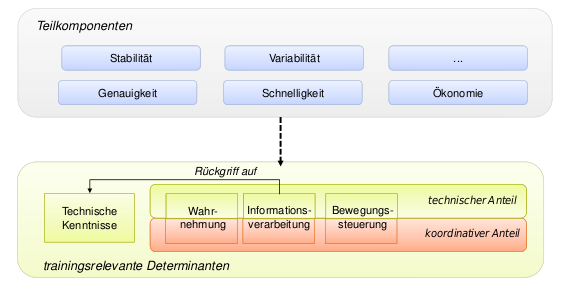
\includegraphics[width=\textwidth]{pictures/tech_determinanten}

\subsubsection*{Phasen des Technikerwerbs}

Das Freiheitsgradproblem:
\begin{itemize}
    \item „Erfunden“ von Nikolai Alexandrowitsch Bernstein, russ. Physiologe, 1896-1966
    \item Problem: Der Mensch hat 880 größere Muskeln!
    \item Wie können diese koordiniert werden?
    \item Motorisches Lernen wird als das Erlernen der Kontrolle von Freiheitsgraden interpretiert: Phasen des motorischen Lernens
\end{itemize}

Phasen des Technikerwerbs:
\begin{enumerate}
    \item Phase ``Freezing'': Einfrieren der Freiheitsgrade
    \begin{itemize}
        \item Freiheitsgrade: Einschränkungen der Muskelgruppen, beteiligter Gelenke, Ausdehnung der Bewegung
        \item Gestalt: geführte Bewegungen, misslingen zunächst öfter
        \item Methodik: Komplexitätsreduktion, Gelegenheit zur Auseinandersetzung geben: Ermüdung, Rückmeldung
    \end{itemize}
    \item Phase ``Releasing'': Befreien der Freiheitsgrade
    \begin{itemize}
        \item Freiheitsgrade:Sukzessives Freisetzen, „selective defrosting“
        \item Gestalt: flüssige, lockere Bewegung, Kombinationen
        \item Methodik: Intensive Rückmeldungen, große Wiederholungszahlen
    \end{itemize}
    \item Phase ``Exploiting'': Ausbeuten der Freiheitsgrade zur Anpassung, Optimierung
    \begin{itemize}
        \item Freiheitsgrade: Ausnutzen, um dynamisches Optimum zu realisieren
        \item Gestalt: oft DVZ, Absprung-, Aushol-, Schlagbewegungen
        \item Methodik: Wann wird zur Ausbeutung gegriffen? Erhöhte Belastung bedenken!
    \end{itemize}
\end{enumerate}

\subsubsection*{Motor Learning}

Lernarten:
\begin{itemize}
    \item Soziales oder Modelllernen: Lernen vom Vorbild, Star, Lehrer, Vormachen-Nachmachen
    \item Versuch-Irrtum-Lernen: Explorierendes Lernen, Implizites Lernen, Bedeutung oft unterschätzt, Anfänger: keine hinreichende Bewegungsvorstellung, Könner: Gegenstand zu differenziert
    \item Lernen durch Einsicht: Zirkel: Instruktion-Durchführung-Ext./Int.Feedback-Bewegungsvorstellung, Umfang und Bedeutung oft überschätzt, Basis des traditionellen methodischen Vorgehens
\end{itemize}

Methodische Übungsreihen (MÜR):
\begin{itemize}
    \item ``Methodische Übungsreihen sind nach methodischen Grundsätzen geordnete Übungsfolgen, die zur Erlernung einer bestimmten motorischen Fertigkeit (Zielübung) ... führen sollen''
    \item Goldstandard des lehrerzentrierten Sportunterrichts
    \item Typen: Aufgliederung in Teilbewegungen, graduelle Annährung, verminderte Lernhilfen
    \item Anordnungsprinzipien: von einfach zu komplex, von leicht zu schwer
\end{itemize}

Neue Ansätze im motorischen Lernen:
\begin{itemize}
    \item bisherige Modelle zu kognitionslastig
    \item Wahrnehmng und Kontext zu wenig berücksichtigt
    \item Bewegungen werden als Antworten auf Umweltkonstellationen interpretiert: ``Constraints'': Einschränkungen der Möglichkeiten, ``Affordances'': Bewegungsmöglichkeiten, diese Wahrnehmung überwiegend unbewusst
    \item Systemdynamischer Ansatz:
    \begin{itemize}
        \item es gibt keine zentrale kortikale Kontrollinstanz zur Bewegungssteuerung
        \item folglich bilden bewusste Prozesse lediglich einen Rahmen für die Bewegungsausführung und sind für die Bewegungskontrolle wenig bedeutsam
        \item Kontrolle wird an dezentrale ``koordinative Strukturen'' delegiert
    \end{itemize}
    \item Ecological approaches: Bewegug wird in einem chaotischen Prozess und in Abhängigkeit von den wechselnden Umweltbedingungen meist unbewusst jedes mal neu generiert. Bewegungslernen = unbewusste Selbstorganisationsprozesse
    \item Implizites Lernen:
    \begin{itemize}
        \item unbewusstes Lernen, ohne Aufmerksamkeit
        \item inzidentell: Unbeabsichtiges Lernen durch Konfrontation mit Lernsituation, Erfolg nicht herbeiführbar (Straßenfußballer-Hypothese)
        \item erfordert intensive und umfangreiche Beschäftigung und hohe Motivation
        \item experimentelle Befunde in der Psychologie
        \item besonders geeignet für komplexe und nicht zu verbalisierende Lerngegenstände
    \end{itemize}
\end{itemize}

Indikationen:
\begin{description}
    \item [Explizit / intentional] bewusstseinspflichtige (erste Lernphasen?) und bewusstseinsfähige Inhalte (Spielzüge, Konzeptionen, Standardsituationen), besonders in kompositorischen und konditionellen Sportarten
    \item [Implizit / inzidentell] komplexe und immer neue Situationen, besonders Sportspiele und Kampfsportarten
\end{description}

\subsection{Trainingsmethoden}

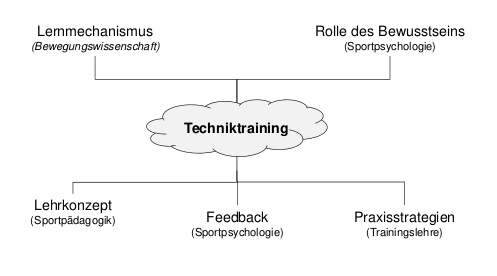
\includegraphics[width=\textwidth]{pictures/tech_mindmap}

\subsubsection*{Lernmechanismus (Bewegungswissenschaft)}

Theorien zum motorischen lernen (die zweite):
\begin{itemize}
    \item Operande Konditionierung (Skinner, 1955): ML ist das Antrainieren von Reflexen auf Umweltreize
    \item Freezing, Releasing, Exploiting (Bernstein,1967): ML ist die Kontrolle von Freiheitsgraden
    \item Motorisch Programme (Schmidt, 1974): ML ist der Aufbau von zentral steuerbaren motorischen Programmen
    \item Theorie der Sensomotorik (Ungerer, 1977): ML ist das Verknüpfen „motorischer Elementarzeichen“ zu Bewegungssequenzen
    \item Ökologische Ansätze (Gibson, 1979, Turvey, 1977): ML ist ein unbewusster Selbstorganisationsvorgang als Antwort auf Umweltwahrnehmungen
\end{itemize}

Lernen durch \ldots:
\begin{itemize}
    \item Konditionierung: Antrainieren von Reflexen (z.B. Deckung beim Boxen), Abtrainieren (Habituation) von Reflexen (z.B. Handballtorwart), Einüben von Bewegungsrhythmen (Stemmschritt)
    \item Imitation: z.B. Fotos, Bildreihen, Videoaufnahmen, Vormachen des Trainers, Beobachtung von anderen Sportlern
    \item Einsicht: Gedankliche Auseinandersetzung mit der eigenen Bewegung, Suchen nach und Erkennen von Fehlern, Erfassen von Ursache und Wirkung, Erarbeitung einer Lösung
    \item Versuch und Irrtum: Lernen muss weitgehend ohne externe Kontrolle/Korrektur funktionieren (z.B. Muttersprache, grundlegende Motorik), Motivation ist nicht das Lernen an sich sondern die Erreichung eines Zieles, Selbständiges Suchen nach Lösungen, Rückschläge in Kauf nehmen, Lernen geschieht hierbei nebenläufig und unbewusst (implizit)
\end{itemize}

\subsubsection*{Lehrkonzept (Sportpädagogik)}

Explizites Techniklernen:
\begin{itemize}
    \item Technik wird wie ein Produkt in mehreren Schritten bewusst (=intentional) ``hergestellt'' (=technologische Position)
    \item Lernen durch Konditionierung, Einsicht, Modellernen, extrinsisches Feedback
    \item Gedankliche Erfassung der Bewegung $\rightarrow$ Beherrschen der Grobform $\rightarrow$ Variation, Stabilisation, Abschirmung
    \item Kritik: ``Kids in America grow up playing in the parks. In Germany they come to the clubs and have practice and stuff like that!''
\end{itemize}

Implizites Techniklernen:
\begin{itemize}
    \item Beiläufiges, ``natürliches'' Lernen ohne Lernabsicht am Einzelfall (=inzidentell)
    \item Antrieb ist eine realen Situation zu lösen
    \item intensive und umfangreiche Beschäftigung, höchst motiviert
    \item Lernen durch Versuch \& Irrtum
    \item ``Freies, unangeleitetes Spielen führt zu Verbesserungen der technischen und taktischen Leistungsvoraussetzungen und ist expliziten Methoden teilweise sogar überlegen'' (Straßenspielerhypothese)
    \item Kritik: Straßenspiel ist zu wenig steuerbar, zu langsam, Erfolg ist unsicher
\end{itemize}

\subsubsection*{Rolle des Bewusstseins (Sportpsychologie)}

\begin{description}
    \item [bewusstseinspflichtige Inhalte] leicht verbalisierbare und vermittelbare Inhalte ( z.B. Regelvorgaben für Techniken)
    \item [bewusstseinsfähige Inhalte] nicht immer bewusst aber bei besonderer Aufmerksamkeit wahrnehmbar \& ansteuerbar (z.B. Technikknotenpunkte), Sprachliche Repräsentation meist schwierig aber lernbar
    \item [nicht bewusstseinsfähige Inhalet] Prozesse die nicht zentral wahrgenommen werden (z.B. propriorezeptive Informationen, intermuskuläre Koordination, Entstehen von Innervationsmustern) - nicht Teil der technischen Kenntnisse
\end{description}

Top-Down vs. Bottom-Up:
\begin{description}
    \item [Top-Down] Willkürlich, gedankliche Kontrolle der Bewegung, bewusstes Ansteuern von Inhalten
    \item [Bottom-Up] Unwillkürlich, Nur Anstoß zur Bewegung erfolgt bewusst, Kontrolle erfolgt unbewusst ohne Aufmerksamkeit (``automatisch'')
\end{description}
\begin{itemize}
    \item Top-Down kann Bottom-Up beliebig überlagern (explicit monitoring, conscious processing)
    \item Bewegung langsamer und weniger flüssig (Constrained Action-Hypothese; Wulf), Möglicher Grund: Differenzbildung ( ->Antizipative Verhaltenskontrolle)
    \item In ersten Lernphasen hilfreich um Bewegung selber zu korrigieren (Technikknotenpunkte)
    \item externe vs. internale Fokussierung (Bewegung des Schlägers vs. Bewegung der Arme)
    \item Dynamisches Optimum nur über Bottom-Up- Prozesse möglich?! ABER Genauigkeit bei Top-Down-Prozesse höher?
\end{itemize}

\subsubsection*{Feedback (Sportpsychologie)}

Feedback:
\begin{itemize}
    \item Informationen über die Bewegungsrealisation
    \item Limitation intrinsisches Feedback: Sensibilität des Übenden, sensorisches Feedback kann nciht interpretiert werden!, nicht überprüfbar
    \item Extrensisches Feedback:
    \begin{itemize}
        \item kann fördern wenn Sensorik beeinträchtigt oder Erfahrungen zur Interpretation fehlen
        \item oder behindern wenn Durchführung gestört wird,  (richtige) eigene Wahrnehmung durch eine (falsche) Information in den Hintergrund gedrängt wird,  Abhängigkeit von Feedback erzeugt wird oder das Feedback als Kritik wahrgenommen wird
        \item Umfang: Nicht jeden Übungsversuch (30\%) und nur schwerwiegende Fehler korrigieren. Bei Anfängern zunächst nur den Hauptfehler korrigieren. Leitsatz: soviel extrinsisches Feedback wie nötig, soviel intrinsisches Feedback wie möglich
        \item Inhalte: knowledge of result (Bewegungsergebnis), knowledge of performance (Bewegungsausführung), Fehler effektiver, Richtiges motivierender (4:1? Siedentop, 1983), Fehler und Ursachen kurz und präzise beschreiben, Direkte Umsetzbarkeit des Feedbacks in motorische Handlung, Negationen vermeiden, Maximal zwei Information pro Korrektur
    \end{itemize}
    \item Zeitpunkt: Bewegungsempfindungen verblassen nach der Bewegung kontinuierlich, deshalb Feedback rechtzeitig (5-30s) geben. Nach der Korrektur genügend Zeit bis zum nächsten Versuch einräumen (>15s). Keine anderen Bewegungsaufgaben zwischen Feedback und erneutem Versuch
\end{itemize}

\subsubsection*{Praxisstrategien (Trainingslehre)}

Erwerben:
\begin{itemize}
    \item analytisch-synthetisch, ganzheitlich-graduell oder ganzheitlich?
    \item Argumente für schrittweises Lernen: Zahlreiche zu viele Teilbewegungen gleichzeitig oder nacheinander, Technik erfordert zu viel Kraft oder Schnelligkeit, schnell wechselnde, nicht konstante Situationen, zu hoher Zeitdruck, nicht ausreichende Wahrnehmung der eigenen Bewegung $\rightarrow$ Techniken können meist nicht direkt und ganzheitlich vermittelt werden
    \item Methodische Übungsreihe: ``Systematische kleinschrittige Übungsfolgen zum Aufbau sporttypischer Bewegungstechniken, die verschiedenen Vereinfachungsmaßnahmen miteinander verbinden'', erst vereinfachen, dann Vereinfachung zurücknehmen
    \item Reduktion des Bewegungsumfangs: Aufgliedern in Teilbewegungen, Lernen der Teilbewegungen, Zusammensetzen der Teilbewegungen
    \item Reduktion Bewegungslänge: Mögliche bei nacheinander realisierbaren Bewegungsteilen (zyklisch nein, azyklisch ja), dabei Wurf- oder Stoßbewegungen auf Wechselwirkungen prüfen, Ersatz für fehlende Teilbewegungen notwendig
    \item Reduktion Bewegungsbreite: Sinnvoll bei wenig Wechselwirkung zwischen Teilen (synchron nein, alternierend ja), Ersatz für fehlende Teilbewegungen notwendig (z.b. Schwimmbretter)
    \item Reduktion Präzisionsdruck: Erhöhung der Fehlertoleranz durch Regeländerungen
    \item Reduktion Geschwindigkeits- und Zeitdruck: Zeitanforderung (Verlängerung der möglichen Bewegungsdauer, z.b. Trampolineinsatz, springen von Kästen) oder Bewegungsgeschwindigkeit (Verlangsamung von Teilbewegungen)
    \item Reduktion Kraftanforderung: Verringerung des Bewegungswiderstandes (z.B. Hilfestellung, leichte Wurfgeräte, ...)
    \item Visuelle Lernhilfen: Bewegungstechniken während Demonstration beschreiben und erklären, eindeutige Bewegungsmerkmale hervorheben, Demonstration langsam aber nicht Dynamik verfälschen, Orientierungspuntke
    \item Akustische Lernhilfen: Vorgabe von Rhythmen oder Bewegungsdynamik
    \item Taktile Lernhilfen: Bewusstmachen von Trajektorien und Winkelstellungen
\end{itemize}

Variationstraining:
\begin{itemize}
    \item Variabilität = willkürliche Veränderung der Bewegungsausführung
    \item Wichtig bei offenen Fertigkeiten (Sportspiele, Kampfsport)
    \item explizit trainieren, dabei Variabilität beschränken, z.B. nur ein Merkmal gleichzeitig variieren ( z.B. Veränderung der Schrittzahl beim Sprungwurfanlauf, Wurfrichtung konstant) oder mehrere Merkmale variieren, aber den Variationsumfang beschränken (z.B. nur 2 oder 3 Schritte, nur zwei Wurfrichtungen)
    \item Voraussetzung Automatisierung(?) = Bewegungsausführung mit reduzierter Aufmerksamkeit
    \item Ressourcentheorie: freiwerdende Ressourcen können für Wahrnehmung und gezielte Variationen genutzt werden, deshalb Zusatzaufgaben, die Aufmerksamkeit von der Hauptaufgabe weglenken
\end{itemize}

Stabilisierungstraining:
\begin{itemize}
    \item Stabilisierung = Eingrenzen der Varianz bei Bewegungsausführung und Ergebnis
    \item Wichtig bei geschlossenen Fähigkeiten (Leichtathletik, Turnen)
    \item Ansatz 1: Verbesserung von Bewegungsvorstellung - Feedback über Bewegungsergebnisse und Qualität
    \item Ansatz 2: Anpassungstraining = Erhöhung des Anpassungsdrucks durch veränderte Wahrnehmungs- und Umweltbedingungen
\end{itemize}

Abschirmungstraining: Training unter erschwerten
Umweltbedingungen (Bsp: 1. Konditionelle Vorermüdung (Handball auf Sand), 2. Gegnereinwirkung (Flanke gegen Gegner durchsetzen), 3. Psychischer Druck (Sanktionen bei Fehlern)

\subsection{Trainingsinhalte}

Durch Übungsgestaltung sicherstellen, dass Situation entstehen, in der die Technik unter dem intendierten Aspekt angewendet werden kann/muss. Mit steigendem Niveau Zieltechnik unter verschiedenen Aspekten durchführen! und verschiedenen Situationen explizit trainieren (ualitätsgesetz).
Ziele dabei möglichst konkret formulieren.
Ansonsten sehr sportartspezifisch (siehe sportpraktische Veranstaltungen).

\subsection{Anwendung}

Zusammenfassung Kenntnisstand:
\begin{itemize}
    \item ``Harte'' wissenschaftliche Fakten zur Begründung Mangelware
    \item Weniger „Schuld“ der Wissenschaft als vielmehr Natur eines komplexen Phänomens
    \item Pragmatisch erfolgt die Ableitung von Empfehlungen auf Basis von Hypothesen, abgeleitet aus Theorien der Basiswissenschaften, rational begründeten Verfahren der Sportpraxis oder Erfahrungen der Sportpraxis
\end{itemize}

Indikationen für Lernverfahren:

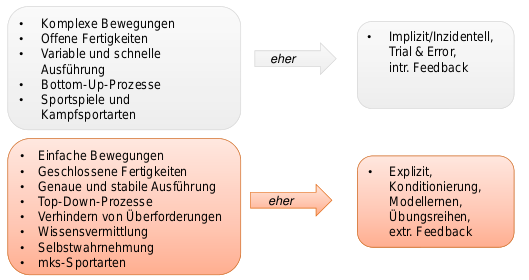
\includegraphics[width=\textwidth]{pictures/tech_lernverfahren}

\subsection{Diagnostik}

Varianten:
\begin{description}
    \item[Videoanalyse] Bildreihen, Videoaufnahmen, Qualitative Bewertung, Hochfrequenzaufnahmen
    \item [Motion Capturing] 1. Aufnahme mit mehreren Videokameras, 2. Fitting eines Körpermodells, 3. Berechnung biomechanischer Kenndaten aus dem Körpermodell (Verlauf in Raum und Zeit, Gelenkwinkel)
    \item [Kraft- und Beschleunigungssensorik]
    \item [Geschwindigkeitsmessung] Radarmessung
\end{description}

\subsection{Zusammenfassung}

\begin{itemize}
    \item Explizite Verfahren eher zum Neulernen oder bei einfachen, langsamen Bewegungen
    \item Bei komplexen, schnellen Bewegungen Rahmenbedingungen schaffen, das Selbstorganisationsprozessen erfolgen können
    \item Methodische Übungsreihen/ Spielreihen einsetzen um Überforderungen zu vermeiden
    \item Explizit wahrscheinlich überschätzt
\end{itemize}
